\section{Date: 2026-10-08}
\noindent \textbf{Series ID: FORLTCORPPOS42005} 

\noindent This series is titled Foreign Portfolio Holdings of U.S. Long-Term Corporate Bonds: Hong Kong and has a frequency of Monthly. The units are Millions of Dollars and the seasonal adjustment is Not Seasonally Adjusted.The observation start date is 1984-12-01 and the observation end date is 2026-07-01.The popularity of this series is 2. \\ 

\noindent \textbf{Series ID: EMISSCO2VNGCCBA} 

\noindent This series is titled Commercial Carbon Dioxide Emissions, Natural Gas (Pipeline) for United States (DISCONTINUED) and has a frequency of Annual. The units are Metric Tons CO2 and the seasonal adjustment is Not Seasonally Adjusted.The observation start date is 1980-01-01 and the observation end date is 2017-01-01.The popularity of this series is 1. \\ 

\subsection{Raw Regression}
\noindent Regresses the two series against each other directly. A significant result here can come just as easily from both series sharing a long-run trend as from any real relationship.

\begin{center}
\begin{tabular}{lclc}
\toprule
\textbf{Dep. Variable:}                 & value\_fred\_EMISSCO2VNGCCBA & \textbf{  R-squared:         } &     0.242   \\
\textbf{Model:}                         &             OLS              & \textbf{  Adj. R-squared:    } &     0.217   \\
\textbf{Method:}                        &        Least Squares         & \textbf{  F-statistic:       } &     9.875   \\
\textbf{Date:}                          &       Thu, 08 Oct 2026       & \textbf{  Prob (F-statistic):} &  0.00367    \\
\textbf{Time:}                          &           18:03:19           & \textbf{  Log-Likelihood:    } &   -586.01   \\
\textbf{No. Observations:}              &                33            & \textbf{  AIC:               } &     1176.   \\
\textbf{Df Residuals:}                  &                31            & \textbf{  BIC:               } &     1179.   \\
\textbf{Df Model:}                      &                 1            & \textbf{                     } &             \\
\textbf{Covariance Type:}               &          nonrobust           & \textbf{                     } &             \\
\bottomrule
\end{tabular}
\begin{tabular}{lcccccc}
                                        & \textbf{coef} & \textbf{std err} & \textbf{t} & \textbf{P$> |$t$|$} & \textbf{[0.025} & \textbf{0.975]}  \\
\midrule
\textbf{const}                          &    1.558e+08  &     3.05e+06     &    51.049  &         0.000        &      1.5e+08    &     1.62e+08     \\
\textbf{value\_fred\_FORLTCORPPOS42005} &     770.8558  &      245.299     &     3.143  &         0.004        &      270.565    &     1271.147     \\
\bottomrule
\end{tabular}
\begin{tabular}{lclc}
\textbf{Omnibus:}       &  0.800 & \textbf{  Durbin-Watson:     } &    0.469  \\
\textbf{Prob(Omnibus):} &  0.670 & \textbf{  Jarque-Bera (JB):  } &    0.606  \\
\textbf{Skew:}          & -0.321 & \textbf{  Prob(JB):          } &    0.739  \\
\textbf{Kurtosis:}      &  2.832 & \textbf{  Cond. No.          } & 1.69e+04  \\
\bottomrule
\end{tabular}
%\caption{OLS Regression Results}
\end{center}

Notes: \newline
 [1] Standard Errors assume that the covariance matrix of the errors is correctly specified. \newline
 [2] The condition number is large, 1.69e+04. This might indicate that there are \newline
 strong multicollinearity or other numerical problems.

\begin{figure}
\centering
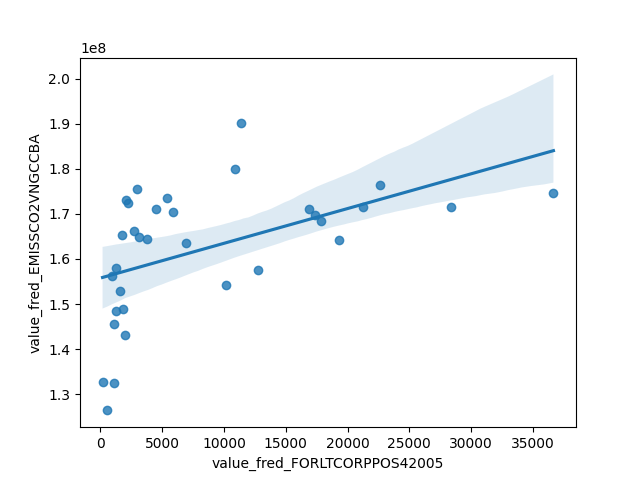
\includegraphics[scale = 0.9]{plots/plot_2026-10-08.png}
\caption{Raw Regression Plot for 2026-10-08}
\end{figure}
\newpage
\subsection{Detrended Regression}
\noindent Regresses the residuals of each series after removing its own linear time trend, so a shared trend can no longer drive the result on its own. A relationship that stays significant here is better evidence of a genuine link between the two series.

\begin{center}
\begin{tabular}{lclc}
\toprule
\textbf{Dep. Variable:}                            & value\_fred\_EMISSCO2VNGCCBA\_detrended & \textbf{  R-squared:         } &     0.247   \\
\textbf{Model:}                                    &                   OLS                   & \textbf{  Adj. R-squared:    } &     0.223   \\
\textbf{Method:}                                   &              Least Squares              & \textbf{  F-statistic:       } &     10.18   \\
\textbf{Date:}                                     &             Thu, 08 Oct 2026            & \textbf{  Prob (F-statistic):} &  0.00324    \\
\textbf{Time:}                                     &                 18:03:19                & \textbf{  Log-Likelihood:    } &   -570.19   \\
\textbf{No. Observations:}                         &                      33                 & \textbf{  AIC:               } &     1144.   \\
\textbf{Df Residuals:}                             &                      31                 & \textbf{  BIC:               } &     1147.   \\
\textbf{Df Model:}                                 &                       1                 & \textbf{                     } &             \\
\textbf{Covariance Type:}                          &                nonrobust                & \textbf{                     } &             \\
\bottomrule
\end{tabular}
\begin{tabular}{lcccccc}
                                                   & \textbf{coef} & \textbf{std err} & \textbf{t} & \textbf{P$> |$t$|$} & \textbf{[0.025} & \textbf{0.975]}  \\
\midrule
\textbf{const}                                     &   -1.899e-06  &     1.39e+06     & -1.37e-12  &         1.000        &    -2.83e+06    &     2.83e+06     \\
\textbf{value\_fred\_FORLTCORPPOS42005\_detrended} &    -895.4645  &      280.652     &    -3.191  &         0.003        &    -1467.857    &     -323.071     \\
\bottomrule
\end{tabular}
\begin{tabular}{lclc}
\textbf{Omnibus:}       &  5.377 & \textbf{  Durbin-Watson:     } &    1.047  \\
\textbf{Prob(Omnibus):} &  0.068 & \textbf{  Jarque-Bera (JB):  } &    3.796  \\
\textbf{Skew:}          & -0.669 & \textbf{  Prob(JB):          } &    0.150  \\
\textbf{Kurtosis:}      &  3.985 & \textbf{  Cond. No.          } & 4.94e+03  \\
\bottomrule
\end{tabular}
%\caption{OLS Regression Results}
\end{center}

Notes: \newline
 [1] Standard Errors assume that the covariance matrix of the errors is correctly specified. \newline
 [2] The condition number is large, 4.94e+03. This might indicate that there are \newline
 strong multicollinearity or other numerical problems.

\begin{figure}
\centering
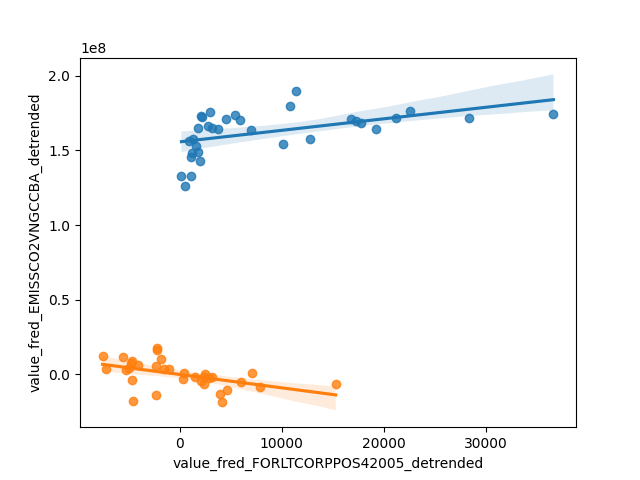
\includegraphics[scale = 0.9]{plots/plot_2026-10-08_detrended.png}
\caption{Detrended Regression Plot for 2026-10-08}
\end{figure}
\newpage
